\begin{name}
	{\tenchude}
	{TOÁN 10}
	{LỚP TOÁN THẦY PHÁT}
	{Life always offers you a second chance. It’s called tomorrow}
\end{name}
\Opensolutionfile{ansbook}[ans/ansbookDe5]
\TN
\Opensolutionfile{ans}[ans/ansDe5-TN1]
\begin{ex}%[0D3H1-5]
Cho hàm số $ f(x) = \sqrt{x^2 - 2x + 5} $. Mệnh đề nào sau đây là mệnh đề đúng?
\choice
{Hàm số nghịch biến trên khoảng $(1;3)$}
{\True Hàm số đồng biến trên khoảng $(2;3)$}
{Hàm số nghịch biến trên khoảng $(1;2)$}
{Hàm số nghịch biến trên khoảng $(2;3)$}
\loigiai{
Điều kiện xác định của hàm số là $x^2-2x+5\geq 0$ (luôn đúng với mọi $x$).\\
Tập xác định của hàm số là $\mathscr{D}=\mathbb{R}$.\\
Với $x_1$, $x_2$ $\in (1;+\infty)$ và $x_1 < x_2$, ta có
\allowdisplaybreaks
\begin{eqnarray*}
f\left(x_1\right)-f\left(x_2\right)&=& \sqrt{x_1^2 - 2x_1 + 5}-\sqrt{x_2^2 - 2x_2 + 5}\\
&=& \dfrac{x_1^2-2x_1+5-\left(x_2^2-2x_2+5\right)}{\sqrt{x_1^2 - 2x_1 + 5}+\sqrt{x_2^2 - 2x_2 + 5}}\\
&=& \dfrac{\left(x_1-x_2\right)\left(x_1+x_2-2\right)}{\sqrt{x_1^2 - 2x_1 + 5}+\sqrt{x_2^2 - 2x_2 + 5}}>0
\end{eqnarray*}
Vậy hàm số luôn đồng biến trên $(1;+\infty)$ hay hàm số đồng biến trên khoảng $(2;3)$.
}
\end{ex}

\begin{ex}%[Đề kiểm tra HK1 môn Toán 10 Sở giáo dục Bắc Giang]%[Nguyễn Vương Hiển, 10EX-HK1-2223]%[0D3N2-1]
Hàm số nào dưới đây là hàm số bậc hai biến số $x$?
\choice
{$y=\dfrac{x^2+1}{x+1}$}
{$y=\sqrt{3-x^2}$}
{$y=3-x$}
{\True $y=-x^2+2x+5$}
\loigiai{
Hàm số bậc hai biến số $x$ là $y=-x^2+2x+5$.
}
\end{ex}

\begin{ex}%[0D3H2-2]%[Yến Trần]%[Đề cương Nguyễn Thượng Hiền_HK1]
Cho hàm số $y=f(x)=x^2-2x+3$. Trong các khẳng định sau, tìm khẳng định đúng.
\choice
{\True Hàm số nghịch biến trên khoảng $(-\infty;1)$}
{Hàm số đồng biến trên khoảng $(0;+\infty)$}
{Đồ thị hàm số đi qua điểm $A(1;0)$}
{Hàm số đồng biến trên khoảng $(-1;+\infty)$}
\loigiai
{
Ta có $a=1$, $b=-2$, $c=3$ nên $-\dfrac{b}{2a}=-\dfrac{-2}{2 \cdot 1}=1$.\\
Do hệ số $a>0$ nên ta có bảng biến thiên
\begin{center}

\begin{tikzpicture}[>=stealth]
\tkzTabInit[nocadre=false,lgt=1,espcl=2,deltacl=0.5]{$x$/.7 ,$y$/2}
{$-\infty$ , $1$ , $+\infty$}
\tkzTabVar{+/$+\infty$ , -/$2$ , +/$+\infty$}
\end{tikzpicture}
\end{center}
Suy ra hàm số nghịch biến trên khoảng $(-\infty;1)$.
}
\end{ex}

\begin{ex}  :%[0D6H1-1]
Các nhà toán học cổ đại Trung Quốc đã dùng phân số $\dfrac{22}{7}$ để xấp xỉ số $\pi $. Hãy đánh giá sai số tuyệt đối $\Delta $ của giá trị gần đúng này, biết $3{,}1415<\pi <3{,}1416$.
\choice
{$\Delta <0{,}0012$}
{$\Delta <0{,}0014$}
{\True $\Delta <0{,}0013$}
{$\Delta <0{,}0011$}
\loigiai{
Vì $3{,}1415<\pi<3{,}1416$\\
nên  $\dfrac{22}{7}-3{,}1416<\dfrac{22}{7}-\pi<\dfrac{22}{7}-3{,}1415$.\\
Suy ra $\left|\dfrac{22}{7}-\pi\right|<\dfrac{22}{7}-3{,}1415 \approx 0{,}014$
}
\end{ex}

\begin{ex}%[HK1, THPT Chuyên Hùng Vương - Phú Thọ, 2023-2024]%[Lê Quốc Hiệp, 10-11EX-HK1-2324]%[0D6H4-2]
Mẫu số liệu sau cho biết chiều cao (đơn vị cm) của các bạn trong tổ
\[\begin{array}{llllllll}163 & 159 & 172 & 167 & 165 & 168 & 170 & 161\end{array}\]
Khoảng biến thiên của mẫu số liệu này bằng
\choice
{$11$}
{$10$}
{\True $13$}
{$12$}
\loigiai
{
Sắp xếp mẫu số liệu theo thứ tự không giảm
\[
\begin{array}{llllllll}
159 & 161 & 163 & 165 & 167 & 168 & 170 & 172
\end{array}
\]
Khoảng biến thiên $R=x_8-x_1=172-159=13$.
}
\end{ex}

\begin{ex}%[0D0N1-2]
Tung một đồng xu và một con xúc xắc, nhận được kết quả là mặt xuất hiện trên đồng xu (sấp hay ngửa) và số chấm xuất hiện trên con xúc xắc. Số kết quả có thể xảy ra là
\choice
{$2$}
{$6$}
{$8$}
{\True $12$}
\loigiai{
Đồng xu chỉ có hai mặt sấp hay ngửa.\\
Con xúc xắc số chấm xuất hiện là $1,2,3,4,5,6$.\\
Số kết quả có thể xảy ra là $2\cdot 6=12$.
}
\end{ex}

\begin{ex}%[0D0N1-3]
Gieo ngẫu nhiên $1$ con xúc xắc cân đối, đồng chất $5$ lần. Số phần tử của không gian mẫu là
\choice
{$15625$}
{$11$}
{$30$}
{\True$7776$}
\loigiai{
Số phần tử của không gian mẫu là $n(\Omega)=6^5=7776$.
}
\end{ex}

\begin{ex}%[0H9H3-1]
Vectơ nào dưới đây là một vectơ pháp tuyến của đường thẳng đi qua hai điểm $A(2;3)$ và $B(4;1)$?
\choice
{ $\overrightarrow{n}_{1}=(2;-2)$}
{$\overrightarrow{n}_{2}=(2;-1)$}
{\True$\overrightarrow{n}_{3}=(1;1)$}
{$\overrightarrow{n}_{4}=(1;-2)$}
\loigiai{
Đường thẳng đi qua hai điểm $A(2;3)$ và $B(4;1)$ có vectơ chỉ phương là $\overrightarrow{AB}=(2;-2)$ suy ra một vectơ pháp tuyến là $\overrightarrow{n}=(1;1)$.}
\end{ex}

\begin{ex}%[0H9H3-2]%[Dự án đề kiểm tra Toán Khối 10 CK2 NH23-24-Dot 15- Nguyễn Hoàng Việt]%[THPT Đặng Huy Trứ - Thừa Thiên Huế]
Phương trình tham số của đường thẳng $d$ đi qua điểm $A\,(-1; 2)$ và song song với đường thẳng $\Delta: 3 x-13 y+1=0$ là
\choice
{\True $\heva{&x=-1+13 t \\& y=2+3 t}$}
{$\heva{&x=1+13 t \\& y=-2+3 t}$}
{$\heva{&x=1+3 t \\& y=2-13 t}$}
{$\heva{&x=-1-13 t \\& y=2+3 t}$}
\loigiai{
Từ phương trình đường $\Delta \Rightarrow \overrightarrow{n_{\Delta}}=(3;-13)\Rightarrow \overrightarrow{u_{\Delta}}=(13;3)$.\\
Vì $(d)\parallel \Delta $ nên $\overrightarrow{u_d}=\overrightarrow{u_{\Delta}}=(13;3)$. Lại có đường thẳng $(d)$ đi qua $A\,(-1;2)$ khi đó phương trình tham số của $\Delta $ là
$\heva{&x=-1+13t\\&y=2+3t}$}
\end{ex}

\begin{ex}%[10-11-12EX-HK1-2425]%[Huỳnh Xuân Tín]%[0H9N3-3]
Trong mặt phẳng $Oxy$, cho hai đường thẳng $d_1\colon 2x-y+3=0$ và $d_2\colon x+2y+1=0$. Vị trí tương đối của hai đường thẳng $d_1$ và $d_2$ là
\choice
{\True Vuông góc với nhau}
{Trùng nhau}
{Cắt nhau nhưng không vuông góc với nhau}
{Song song}
\loigiai{Đường thẳng $d_1\colon 2x-y+3=0$ có vectơ pháp tuyến là $\overrightarrow{n}_1=(2;-1)$ và  đường thẳng $d_2\colon x+2y+1=0$ có vectơ pháp tuyến là $\overrightarrow{n}_2=(1;2)$.\\
Ta có  $2\cdot1+(-1)\cdot2=0$ nên $\overrightarrow{n}_1\cdot \overrightarrow{n}_2=0$. Khi đó hai đường thẳng $d_1$ và $d_2$ vuông góc với nhau.}
\end{ex}

\begin{ex}%[0H9N5-1]
Trong mặt phẳng ${Oxy}$, cho elip $ {(E)}:\dfrac{x^{2}}{36}+\dfrac{y^2}{4}=1$. Độ dài trục lớn bằng
\choice
{ \True ${12}$ }
{ ${37}$ }
{ ${36}$ }
{ ${4}$ }
\loigiai{
Ta có $a^2=36 \Rightarrow a=6$. Độ dài trục lớn bằng $2a={12}$.
}\end{ex}

\begin{ex}%[0H9H5-8]
Viết phương trình chính tắc của Parabol biết đường chuẩn có phương trình $x+1=0$.
\choice
{$y^2=2x$}
{\True $y^2=4x$}
{$y=4x^2$}
{$y^2=8x$}
\loigiai{
Phương trình chính tắc của parabol $\left(P\right)\colon y^2=2px$.\\
Đường chuẩn $x+1=0$ suy ra $\dfrac{p}{2}=1$ $\Rightarrow 2p=4$ $\Rightarrow y^2=4x$. Vậy $y^2=4x$.
}
\end{ex}

\TNTF
\begin{ex}%[0D6H4-2]%[CTST - Lớp 10 - Ôn tập cuối học kì 1 - Đề 2]%[Cao Thành Thái]
Cho bảng số liệu sau:\\
\centerline
{
\begin{tabular}{|>{\centering\arraybackslash}p{2cm}|>{\centering\arraybackslash}p{1cm}|>{\centering\arraybackslash}p{1cm}| >{\centering\arraybackslash}p{1cm}| >{\centering\arraybackslash}p{1cm}| >{\centering\arraybackslash}p{1cm}| >{\centering\arraybackslash}p{1cm}|}
\hline
Giá trị & $21$ & $32$ & $18$ & $24$ & $25$ & $26$ \\
\hline
Tần số & $7$ & $6$ & $4$ & $8$ & $6$ & $10$ \\
\hline
\end{tabular}
}
Xét tính đúng sai của các khẳng định dưới đây.
\choiceTF
{Mốt của mẫu số liệu trên là $10$}
{Số trung bình của mẫu số liệu (làm tròn đến hàng phần chục) là $24{,}9$}
{\True Quy tròn giá trị phương sai của mẫu số liệu với độ chính xác $d=0{,}23$ ta được kết quả là $15$}
{\True Sai số tương đối của số quy tròn phương sai đến hàng đơn vị không vượt quá $1\%$}
\loigiai
{
\begin{itemchoice}
\itemch Giá trị có tần số lớn nhất là $26$ nên $M_O = 26$.
\itemch \[\overline{x} = \dfrac{21\cdot 7 + 32\cdot 6 + 18\cdot 4 + 24\cdot 8 + 25\cdot 6 + 26\cdot 10}{40} = \dfrac{199}{8} \approx 24{,}7.\]
\itemch Phương sai của mẫu số liệu là $s^2=15,036\ldots$, quy tròn với độ chính xác $d=0{,}23$ ta được $s^2\approx 15$.\\
\itemch Sai số tương đối của số quy tròn phương sai đến hàng đơn vị là $\dfrac{|15-15,036\ldots|}{15}\approx 0{,}24\% < 1\%$.
\end{itemchoice}
}
\end{ex}

\begin{ex}%[0H9H3-2]
Trong mặt phẳng tọa độ $Oxy$, cho tam giác $ABC$ có $A(1;1)$, $B(2;-2)$, $C(4;2)$.
\choiceTF
{\True Đường thẳng $AB$ vuông góc với đường thẳng $AC$}
{Phương trình đường cao $AH$ là $x+2y+3=0$}
{\True Đường tròn ngoại tiếp tam giác $ABC$ có tâm $I(3;0)$}
{Đường tròn tâm $C$ đi qua điểm $A$ cắt đường thẳng $AB$ tại hai điểm phân biệt}
\loigiai{
\begin{itemchoice}
\itemch Ta có $\overrightarrow{AB}=(1;-3)$, $\overrightarrow{AC}=(3;1)$. Suy ra $\overrightarrow{AB}\cdot\overrightarrow{AC}=0$ nên $AB\perp AC$.
\itemch Vì vectơ $ \overrightarrow{BC}=\left(2;4\right) $ là vectơ pháp tuyến của đường cao $ AH $.\\
Phương trình đường cao $ AH $ là $ x+2y-3=0 $.
\itemch Vì tam giác $ABC$ vuông tại $A$ nên tâm đường tròn ngoại tiếp tam giác $ABC$ là trung điểm $I(3;0)$ của cạnh huyền $BC$.\\
\itemch Đường tròn tâm $C$ đi qua điểm $A$ có bán kính $AC \perp AB$ nên $AB$ là tiếp tuyến của đường tròn đó. Do đó, đường tròn tâm $C$ đi qua điểm $A$ chỉ có một điểm chung với đường thẳng $AB$ là điểm $A$.
\end{itemchoice}
}
\end{ex}

\TNSA
\begin{ex}%[0D3H2-2]%[CTST - Lớp 10 - Ôn tập cuối học kì 1 - Đề 3]%[Nguyễn Mộng Hùng]
\immini[thm]{
Cho hàm số $y=f(x)$ có tập xác định có đồ thị như hình vẽ.
Biết hàm số nghịch biến trên $(a;b)$. Xác định giá trị lớn nhất của $b-a$.
}{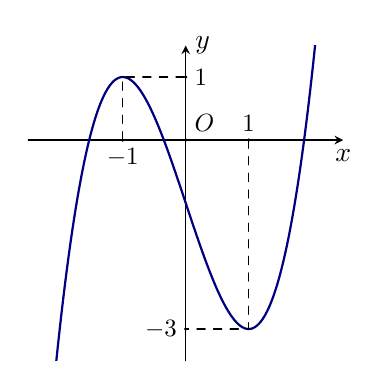
\begin{tikzpicture}[line join = round, line cap = round, >=stealth, scale =.8]
\def\xmin{-2.5}     \def\xmax{2.5}
\def\ymin{-3.5}       \def\ymax{1.5}
\def\f(#1){(#1)^3-3*#1-1}
\draw[->] (\xmin,0)--(0,0) node[above right,scale=.9]{$O$}--(\xmax,0) node[below]{$x$};
\draw[->] (0,\ymin)--(0,\ymax) node[right]{$y$};
\begin{scope}
\clip (\xmin,\ymin) rectangle (\xmax,\ymax);
\draw[smooth, thick, blue!50!black] plot[domain = \xmin:\xmax, samples = 200, variable=\x]({\x},{\f(\x)});
\end{scope}
\foreach \x in {-1,1}{
\pgfmathsetmacro\fx{\f(\x)}
\draw[dashed,thin] (\x,0) |- (0,{\fx});
}
\fill (-1,0)circle (.8pt) node[below,scale=.9]{$-1$};
\fill (1,0)circle (.8pt) node[above,scale=.9]{$1$};
\fill (0,1)circle (.8pt) node[right,scale=.9]{$1$};
\fill (0,-3)circle (.8pt) node[left,scale=.9]{$-3$};
\fill (0,0)circle (.8pt);
\end{tikzpicture}}
\shortans{$2$}
\loigiai{
Hàm số nghịch biến trên $(-1;1)$ và trên các khoảng $(a;b)$ là tập con của $(-1;1)$.\\
Do đó giá trị lớn nhất của $b-a$ là $1-(-1)=2$.
}
\end{ex}

\begin{ex}%[10-11-12EX-HK1-2425]%[Lê Quốc Hiệp]%[0D7V2-7]
Lợi nhuận $T(x)$ của một cơ sở sản xuất khi bán hết $x$ sản phẩm trang trí trong một tuần theo công thức $T(x)=-x^2+40x-309$ với đơn vị tính bằng triệu đồng. Nếu muốn lợi nhuận không dưới $10$ triệu đồng thì số sản phẩm ít nhất của cơ sở sản xuất trong một tuần là bao nhiêu? Biết rằng số sản phẩm được làm ra đều bán hết trong tuần đó.
\shortans[oly]{$11$}
\loigiai
{
Điều kiện để lợi nhuận không dưới $10$ triệu đồng là
\begin{eqnarray*}
& & T(x) \geq 10\\
& \Leftrightarrow & -x^2+40x-309 \geq 10\\
& \Leftrightarrow & -x^2+40x-319 \geq 0\\
& \Leftrightarrow & 11 \leq x \leq 29.
\end{eqnarray*}
Vậy số sản phẩm ít nhất để đảm bảo lợi nhuận không dưới $10$ triệu đồng là $11$ sản phẩm.
}
\end{ex}

\begin{ex}%[dự án HSA, Huỳnh Xuân Tín]%[0H9V4-2]
Đường tròn $(C)$ có tâm $I$ thuộc đường thẳng $d\colon x+3y+8=0$, đi qua điểm $A\left(-2;1\right)$ và tiếp xúc với đường thẳng $\Delta:3x-4y+10=0$. Tính bán kính đường tròn $(C)$.
\shortans[1]{$5$}
\loigiai{
Ta có $I\in d \Rightarrow I(-3m-8;m)$.
\begin{eqnarray*}
&&AI^2=\left[\mathrm{d}(I,\Delta)\right]^2 \text{ (cùng bằng } R^2) \\
& \Leftrightarrow & \left(-3m-6\right)^2+\left(m-1\right)^2=\dfrac{\left[3(-3m-8)-4m+10\right]^2}{3^2+(-4)^2}\\
& \Leftrightarrow & 10m^2+34m+37=\dfrac{169m^2+364m+196}{25}\\
& \Leftrightarrow & 81m^2+486m+729=0\\
& \Leftrightarrow & m=-3.
\end{eqnarray*}
Do đó, đường tròn $(C)$ có $\heva{&\text{tâm } I(1;-3)\\& \text{bán kính } R=AI=\sqrt{(9-6)^2+(-3-1)^2}=5.}$\\
Vậy phương trình đường tròn là ${\left(x-1\right)}^2+{\left(y+3\right)}^2=25$.
}
\end{ex}

\TL
\begin{ex}%[Mức 1]%[Dự án Giảng 10-11 Nhóm Toán & LaTex, Lê Minh Thiện Anh]%[0D3H1-2]
Tìm tập xác định của  hàm số $y=\sqrt{x^2-4x-5}+\dfrac{x-1}{\sqrt{4-x^2}}$.
\loigiai{
Hàm số $y=\sqrt{x^2-4x-5}+\dfrac{x-1}{\sqrt{4-x^2}}$ xác định khi và chỉ khi
\[\heva{&x^2-4x-5 \geq 0 \\ &4-x^2 > 0}.\]
Từ điều kiện thứ hai, ta có $-2 < x < 2$.\\
Từ điều kiện thứ nhất, ta giải bất phương trình $x^2-4x-5 \geq 0$:\\
$(x+1)(x-5) \geq 0 \Leftrightarrow x \leq -1$ hoặc $x \geq 5$.\\
Kết hợp với điều kiện $-2 < x < 2$, ta được $-2 < x \leq -1$.\\
Vậy tập xác định của hàm số đã cho là  $\mathscr{D}=(-2;-1]$.
}
\end{ex}

\begin{ex}%[ID6]%[CTST-Lop12-Ontapcuoihocki1-De4]%[Bùi Lương Phúc]%[2D1C3-6]
Một miếng nhôm có bề ngang $30$\,cm được uốn cong tạo thành máng dẫn nước có diện tích mặt cắt ngang bằng $75\sqrt{3}$ cm$^2$ bằng cách chia tấm nhôm thành $3$ phần bằng nhau rồi gập $2$ bên lại như hình vẽ dưới. Hỏi chiều cao của máng nước bằng bao nhiêu (làm tròn đến hàng phần chục)?
\begin{center}
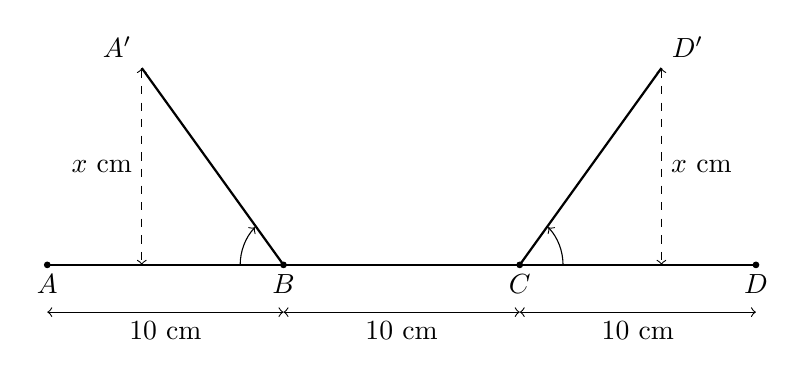
\begin{tikzpicture}
\draw[thick] (0,0) -- (9,0);
\draw[thick] (3,0) -- (1.2,2.5)node[above left]{$A'$};
\draw[thick] (6,0) -- (7.8,2.5)node[above right]{$D'$};
\draw[<->,dashed] (1.2,2.5) -- (1.2,0) node[midway, left] {$x$ cm};
\draw[<->,dashed] (7.8,2.5) -- (7.8,0) node[midway, right] {$x$ cm};
\draw[<->] (0,-0.6) -- (3,-0.6) node[midway, below] {10 cm};
\draw[<->] (3,-0.6) -- (6,-0.6) node[midway, below] {10 cm};
\draw[<->] (6,-0.6) -- (9,-0.6) node[midway, below] {10 cm};
\draw[->] (2.45,0) arc[start angle=180, end angle=137, radius=0.7cm] ;
\draw[->] (6.55,0) arc[start angle=0, end angle=43, radius=0.7cm] ;
\filldraw (3,0) circle (1pt);
\filldraw (6,0) circle (1pt);
\filldraw (0,0) circle (1pt);
\filldraw (9,0) circle (1pt);
\node[below] at (0,0) {$A$};
\node[below] at (3,0) {$B$};
\node[below] at (6,0) {$C$};
\node[below] at (9,0) {$D$};
\end{tikzpicture}
\end{center}
\shortans{1{,}05}
\loigiai
{


}
\end{ex}
\begin{ex}%[Đề phát triển 02]%[Nam Nhất Trần, dự án TeX hóa và phát triển đề tốt nghiệp năm 2025]%[0D0C2-5]
Xung quanh bờ hồ hình tròn, người ta trồng $10$ cây chuối. Người ta chặt ngẫu nhiên $4$ cây chuối.
Tính xác suất để $4$ cây bị chặt không có hai cây nào đứng cạnh nhau.
% \shortans{47}
\loigiai{
\textbf{Cách 1.} \\
Đánh số các cây trên bờ hồ hình tròn từ $1$ đến $10$. \\
Đánh số 4 câu được chọn ngẫu nhiên là $a$, $b$, $c$, $d$ theo thứ tự tăng dần. \\
Số phần tử không gian mẫu là $\mathrm{C}^4_{10}$. \\
Gọi $A$ biến cố thỏa bài toán thì $A$: \lq\lq $1\leq a < b-1 < c-2 < d-3 \leq 7$ \rq\rq.
\begin{itemize}
\item Trường hợp 1. $a=1$. Khi đó $\heva{&b\geq 3 \\&d\leq 9} \Rightarrow \heva{&b-1 \geq 2 \\&d-3 \leq 6.}$ \\
Từ tập $\{2;3;4;5;6\}$, chọn $3$ số và xếp theo tứ tự tăng dần (vào $b-1$, $c-2$, $d-3$), có $\mathrm{C}^3_{5}$ cách. \\
Mỗi cách chọn trên tương ứng với một cách chọn cho $b$, $c$, $d$ thỏa bài toán. \\
Vậy trường hợp này có $\mathrm{C}^3_{5}$ cách.
\item Trường hợp 2. $a\geq 2$. \\
Từ tập $\{2;3;4;5;6;7\}$ chọn 4 số theo và xếp theo thứ tự tăng dần (vào $a$, $b-1$, $c-2$, $d-3$), có $\mathrm{C}^4_{6}$ cách.\\
Mỗi cách chọn trên tương ứng với một cách chọn cho $a$, $b$, $c$, $d$ thỏa bài toán. \\
Vậy trường hợp này có $\mathrm{C}^4_{6}$ cách.
\end{itemize}
Từ hai trường hợp trên suy ra $n(A)=\mathrm{C}^3_{5}+\mathrm{C}^4_{6}=25$ và xác suất của biến cố $A$ là $\mathrm{P}(A)=\dfrac{n(A)}{n(\Omega)}=\dfrac{5}{42}$.
\\
\textbf{Cách 2.} \\
Ta nhắc lại bài toán chia kẹo Euler dạng cơ bản: Phương trình
\[x_1+x_2+...+x_k=n\]
với điều kiện $n\ge k$, có $\mathrm{C}^{k-1}_{n+k-1}$ nghiệm nguyên không âm.
\begin{itemize}
\item Trường hợp 1, giả sử chặt cây $1$. Khi đó cây $2$ và cây $10$ sẽ không bị chặt, vậy ba cây còn lại bị chặt là ba trong số các cây từ $3$ đến $9$. \\
Gọi $x_1$, $x_2$, $x_3$, $x_4$ lần lượt là số lượng cây nằm ở giữa bốn cây bị chặt (chưa bao gồm cây $2$ và cây $10$). \\
Vậy ta có $x_1+x_2+x_3+x_4=4$. Đồng thời $x_1\ge 0$, $x_2\ge 1$, $x_3\ge 1$ và $x_4\ge 0$ (do đã có cây $2$ và cây $10$ đứng cạnh cây $1$ bị chặt, nên $x_1$ và $x_4$ có thể bằng $0$ vẫn thỏa mãn yêu cầu đề bài). \\
Đặt $x_2=y_2+1$, $x_3=y_3+1$, suy ra $x_1+y_2+y_3+x_4=2$ và $x_1,  y_2, y_3, x_4\ge 0$. \\
Áp dụng bài toán chia kẹo Euler, ta có số cách chặt là $\mathrm{C}^3_5=10$ cách.
\item Trường hợp $2$, giả sử cây bị chặt không phải cây $1$. \\
Ta ``trải hình'' thành đường thẳng, duỗi đường tròn tại vị trí cây số $1$. Khi đó, ta xét các cây từ $2$ đến $10$. \\
Ta gọi $x_1$, $x_2$, $x_3$, $x_4$, $x_5$ lần lượt là số cây chưa bị chặt nằm bên trái cây bị chặt số $1$, số cây nằm giữa cây bị chặt $1$ và $2$, số cây nằm giữa cây bị chặt $2$ và $3$, số cây nằm giữa cây bị chặt $3$ và $4$, số cây nằm bên phải cây bị chặt số $4$. \\
Vậy ta có $x_1+x_2+x_3+x_4+x_5=5$ (do từ $2$ đến $10$ có $9$ cây, chặt mất $4$ cây nên còn $5$ cây). \\
Ngoài ra, ta có $x_2, x_3, x_4\ge 1$, đồng thời $x_1\ge 0$ và $x_5\ge 0$. \\
Đặt $x_2=y_2+1$, $x_3=y_3+1$, $x_4=y_4+1$, ta có $x_1+y_2+y_3+y_4+x_5=2$ và $x_1,y_2,y_3,y_4,x_5\ge 0$. \\
Áp dụng bài toán chia kẹo Euler, ta có số cách chặt cây là $\mathrm{C}^4_6=15$ cách.
\end{itemize}
Vậy có $25$ cách chặt thỏa mãn yêu cầu, suy ra xác suất cần tính là $\dfrac{25}{\mathrm{C}^4_{10}}=\dfrac{5}{42}$.
}
\end{ex}
\Closesolutionfile{ans}
\Closesolutionfile{ansbook}
